\documentclass[hyperref={bookmarks=false},aspectratio=169]{beamer}
\usepackage{hyperref,ragged2e,amsmath,amssymb,url,bm}
\usepackage{graphicx,booktabs,array}
\usepackage{tikz}
\usetikzlibrary{arrows.meta,positioning,calc,shapes.geometric,decorations.pathreplacing,matrix}
\graphicspath{{crops/}}
\usetheme{Goettingen}
% --- Paleta "Israel": café ladrillo (ladrillos de Egipto, Éx 1:14), oro del santuario, piedra de Jerusalén ---
\definecolor{cafe}{RGB}{96,52,30}
\definecolor{cafeosc}{RGB}{50,25,13}
\definecolor{tinta}{RGB}{44,28,18}
\definecolor{oro}{RGB}{196,148,40}
\definecolor{ladrillo}{RGB}{158,70,40}
\definecolor{piedra}{RGB}{240,228,203}
\definecolor{sepia}{RGB}{104,86,62}
\setbeamercolor{structure}{fg=ladrillo}
\setbeamertemplate{sidebar canvas right}[vertical shading][top=ladrillo!92!black,bottom=cafeosc]
\setbeamercolor{title in sidebar}{fg=oro}
\setbeamercolor{author in sidebar}{fg=piedra}
\setbeamercolor{section in sidebar}{fg=piedra}
\setbeamercolor{section in sidebar shaded}{fg=oro!60!piedra!70!cafe}
\setbeamercolor{subsection in sidebar}{fg=piedra}
\setbeamercolor{subsection in sidebar shaded}{fg=oro!60!piedra!70!cafe}
\let\raggedright\justifying
\setbeamertemplate{background canvas}{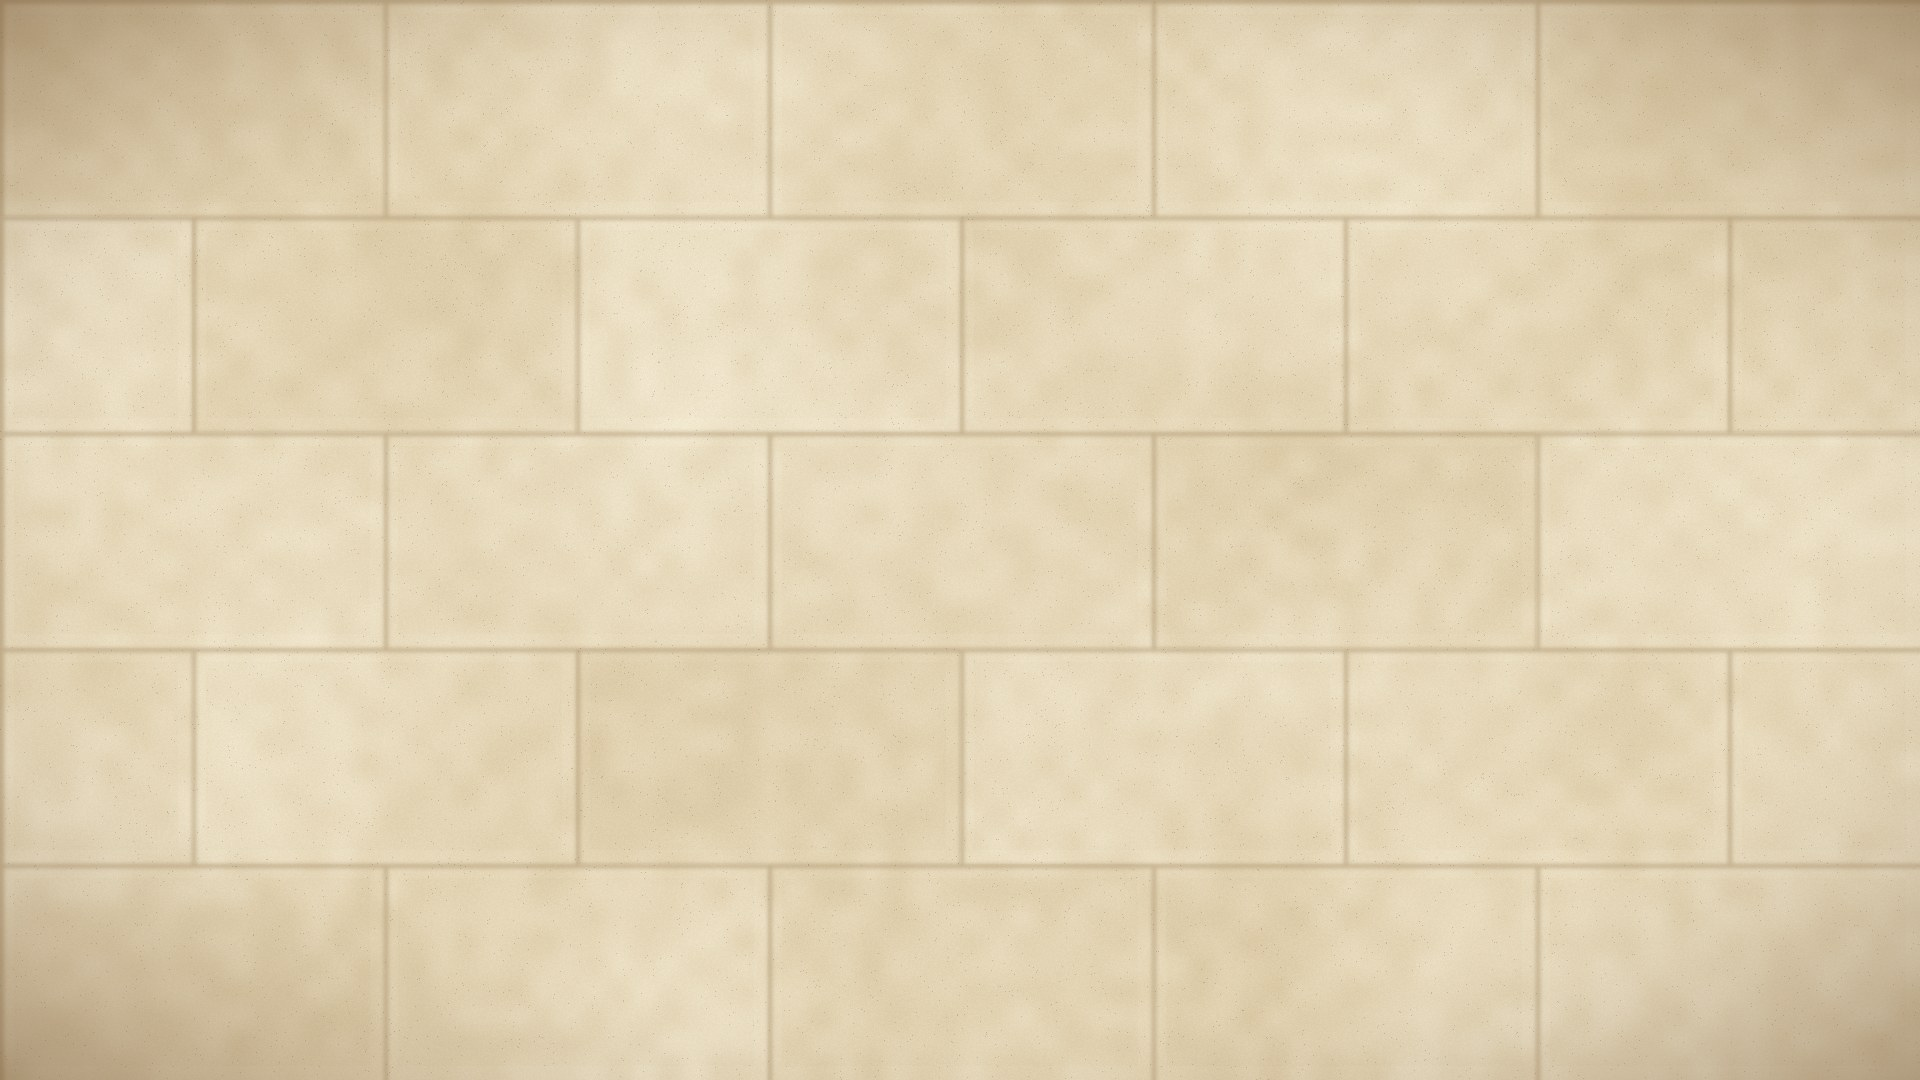
\includegraphics[width=\paperwidth,height=\paperheight]{piedra.jpg}}
\setbeamercolor{normal text}{fg=tinta}
\setbeamercolor{frametitle}{fg=ladrillo}
\setbeamerfont{frametitle}{series=\bfseries}
\setbeamertemplate{section in toc shaded}{\leavevmode{\color{sepia!85!black}\inserttocsection}\par}
\setbeamercolor{title}{fg=ladrillo}
\setbeamercolor{subtitle}{fg=cafe}
\setbeamercolor{item projected}{bg=cafe,fg=piedra}
\setbeamertemplate{itemize item}{\small\textcolor{oro!85!ladrillo}{$\blacktriangleright$}}
\setbeamertemplate{navigation symbols}{}
% --- Español + hebreo + griego (XeLaTeX) con fuentes empaquetadas en fonts/ ---
\usepackage[bidi=default]{babel}
\babelprovide[import,main]{spanish}
\babelprovide[import]{hebrew}
\babelprovide[import]{ancientgreek}
\babelfont[hebrew]{sf}[Path=fonts/, BoldFont=NotoHebrewSans-700.ttf]{NotoHebrewSans-400.ttf}
\babelfont[hebrew]{rm}[Path=fonts/, BoldFont=NotoHebrewSans-700.ttf]{NotoHebrewSans-400.ttf}
\babelfont[ancientgreek]{sf}[Path=fonts/]{GFSPorson.otf}
\babelfont[ancientgreek]{rm}[Path=fonts/]{GFSPorson.otf}
\newcommand{\heb}[1]{\mbox{\foreignlanguage{hebrew}{#1}}}
\newcommand{\grc}[1]{\foreignlanguage{ancientgreek}{#1}}
% --- Citas, imágenes, referencias ---
\usepackage[most]{tcolorbox}
\newtcolorbox{cita}[1][]{enhanced, colback=piedra!92!white, colframe=ladrillo!85!oro,
  boxrule=0pt, leftrule=2.5pt, arc=0pt, left=6pt, right=6pt, top=4pt, bottom=4pt,
  before skip=4pt, after skip=6pt, fontupper=\small\itshape, #1}
\newcommand{\fuente}[1]{\par\hfill{\upshape\bfseries\footnotesize\textcolor{ladrillo}{#1}}}
\newcommand{\imagen}[3][0.80]{%
  \centering\includegraphics[height=#1\textheight,width=\linewidth,keepaspectratio]{#2}\par\vspace{2pt}
  {\fontsize{5}{6}\selectfont\color{sepia}{\raggedleft\textit{Nota.} #3\par}}}
\makeatletter
\newcommand{\fotolado}[2]{%
  \begin{tikzpicture}[remember picture,overlay]
    \node[anchor=north east,inner sep=0pt] (foto) at ([xshift=-\beamer@sidebarwidth]current page.north east)
      {\includegraphics[height=\paperheight]{#1}};
    \node[anchor=south east,inner sep=2pt,text=piedra,fill=cafeosc,fill opacity=0.6,text opacity=1,
      font=\fontsize{4.5}{5.5}\selectfont,align=right,text width=4.2cm] at ([xshift=-3pt,yshift=3pt]foto.south east)
      {\textit{Nota.} #2};
  \end{tikzpicture}}
\makeatother
\newcommand{\refapa}[1]{\par\hangindent=1.2em\hangafter=1\noindent #1\par\vspace{3pt}}
\usepackage{xurl}\urlstyle{same}
\newcommand{\destacar}[1]{\textbf{\textcolor{ladrillo}{#1}}}
\usetikzlibrary{shadows}
\tikzset{caja/.style={draw=cafe!80!black,line width=0.7pt,top color=piedra!55!white,bottom color=piedra!92!oro,
  rounded corners=4pt,inner sep=5pt,font=\scriptsize,
  drop shadow={shadow xshift=0.7pt,shadow yshift=-0.8pt,opacity=0.25,fill=cafeosc}},
  >={Stealth[length=2.4mm,width=1.8mm]}, every picture/.style={line cap=round,line join=round}}
\newcommand{\precision}[1]{{\footnotesize\color{sepia}\textbf{Precisión:} #1}}
\newcommand{\pt}[2]{({#1-30},{#2-29})}
\title[Israel 2: Éxodo--Josué]{\bfseries{Israel, el pueblo de Dios}}
\subtitle{Estudio 2. Del Éxodo a la muerte de Josué}
\author{}\institute{}\date{}
\titlegraphic{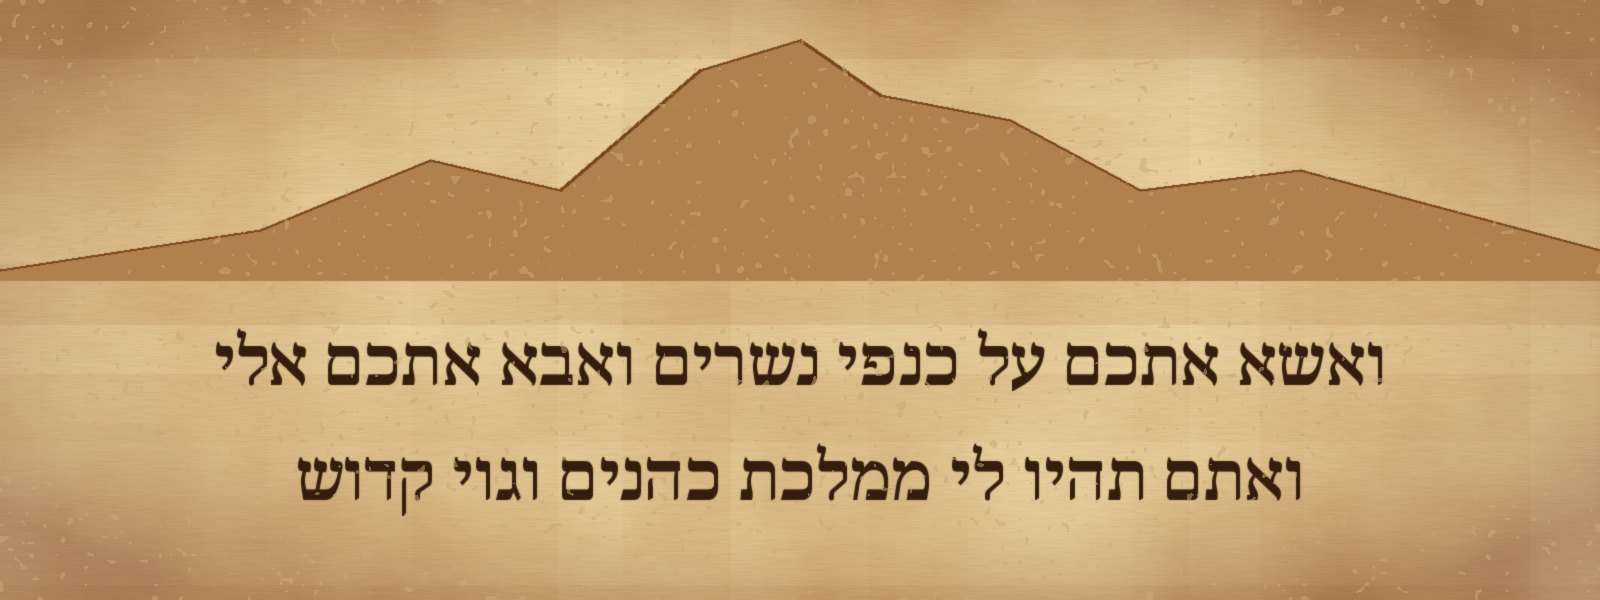
\includegraphics[width=0.85\linewidth,height=0.38\textheight,keepaspectratio]{portada.jpg}\\[-1pt]
  {\fontsize{5}{6}\selectfont\color{sepia}\textit{Nota.} Elaboración propia: Éx 19:4b y 19:6a en texto hebreo consonántico (BHS).}}
\AtBeginSection[]{\begin{frame}\frametitle{Contenidos}\tableofcontents[currentsection]\end{frame}}
\begin{document}
\frame{\titlepage}
\begin{frame}\frametitle{Contenidos}\tableofcontents\end{frame}

% ===================================================
\section{Introducción}
\begin{frame}{¿Qué hace de esclavos un pueblo?}
\begin{columns}[t,onlytextwidth]
\begin{column}{0.52\textwidth}
\begin{cita}Vosotros me seréis un reino de sacerdotes y una nación santa.\fuente{(Éx 19:6)}\end{cita}
\begin{cita}De ellos son la adopción, la gloria, los pactos, la promulgación de la ley, el culto y las promesas.\fuente{(Ro 9:4)}\end{cita}
\end{column}
\begin{column}{0.45\textwidth}\small\RaggedRight
Salir de Egipto no basta: en el Sinaí, tres meses después, Dios revela para qué liberó a Israel.\par\medskip
\destacar{El pacto.} La vocación sacerdotal toma forma de pacto: redención antes de la ley (Éx 20:2), Dios en medio del pueblo (Éx 25:8), Torá como sabiduría ante los pueblos (Dt 4:6).\par\medskip
\destacar{Ruptura y promesa.} La misma etapa que rompe el pacto guarda los textos de restauración más claros de la Torá (Éx 34:6--7; Dt 4:25--31; 30:1--10).
\end{column}
\end{columns}
\end{frame}

\begin{frame}{Los ejes de la serie en esta etapa}
\centering
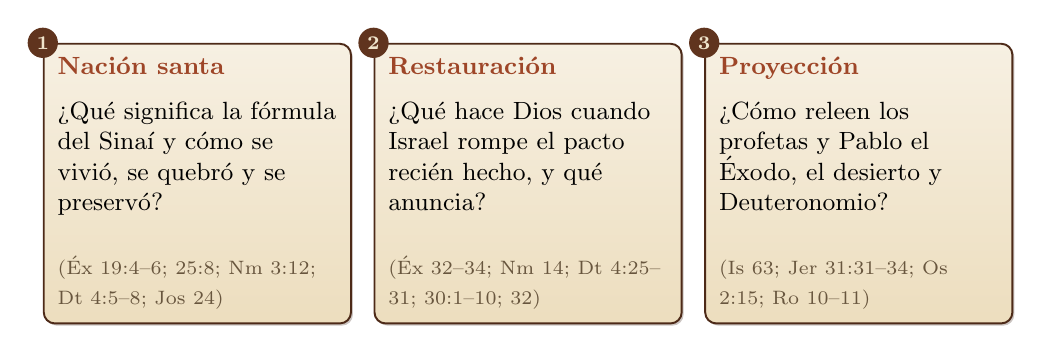
\begin{tikzpicture}
 \foreach \x/\n/\t/\d/\r in {0/1/{Nación santa}/{¿Qué significa la fórmula del Sinaí y cómo se vivió, se quebró y se preservó?}/{Éx 19:4--6; 25:8; Nm 3:12; Dt 4:5--8; Jos 24},
   4.2/2/{Restauración}/{¿Qué hace Dios cuando Israel rompe el pacto recién hecho, y qué anuncia?}/{Éx 32--34; Nm 14; Dt 4:25--31; 30:1--10; 32},
   8.4/3/{Proyección}/{¿Cómo releen los profetas y Pablo el Éxodo, el desierto y Deuteronomio?}/{Is 63; Jer 31:31--34; Os 2:15; Ro 10--11}}{
  \node[caja,anchor=north] (b\n) at (\x,0) {\parbox[t][3.2cm][t]{3.55cm}{\RaggedRight
    {\small\textbf{\textcolor{ladrillo}{\t}}}\\[5pt]\small \d\par\vfill{\scriptsize\color{sepia}(\r)}}};
  \node[circle,fill=cafe,text=piedra,font=\scriptsize\bfseries,inner sep=1.6pt] at (b\n.north west) {\n};}
\end{tikzpicture}\par\vspace{6pt}
{\scriptsize\color{sepia}Las citas bíblicas son traducción propia desde el texto hebreo (BHS) y griego (NA28). Numeración española [hebrea] cuando difiere.}
\end{frame}

% ===================================================
\section{Cronología}
\begin{frame}{Secuencia de la etapa}
\centering
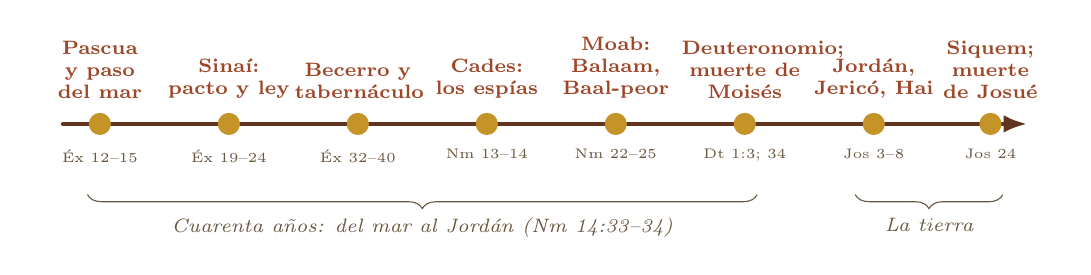
\begin{tikzpicture}[x=0.78cm]
\draw[line width=1.6pt,cafe,-{Latex[length=3mm]}] (0,0) -- (15.7,0);
\foreach \x/\t/\b in {0.6/{Pascua y paso del mar}/{Éx 12--15},
                      2.7/{Sinaí: pacto y ley}/{Éx 19--24},
                      4.8/{Becerro y tabernáculo}/{Éx 32--40},
                      6.9/{Cades: los espías}/{Nm 13--14},
                      9.0/{Moab: Balaam, Baal-peor}/{Nm 22--25},
                      11.1/{Deuteronomio; muerte de Moisés}/{Dt 1:3; 34},
                      13.2/{Jordán, Jericó, Hai}/{Jos 3--8},
                      15.1/{Siquem; muerte de Josué}/{Jos 24}}{
  \fill[oro] (\x,0) circle (4pt);
  \node[above,font=\scriptsize\bfseries,text=ladrillo,text width=1.6cm,align=center] at (\x,0.2) {\t};
  \node[below,font=\tiny,text=sepia,text width=1.6cm,align=center] at (\x,-0.2) {\b};}
\draw[decorate,decoration={brace,amplitude=5pt,mirror},sepia] (0.4,-0.9) -- (11.3,-0.9) node[midway,below=5pt,font=\scriptsize\itshape]{Cuarenta años: del mar al Jordán (Nm 14:33--34)};
\draw[decorate,decoration={brace,amplitude=5pt,mirror},sepia] (12.9,-0.9) -- (15.3,-0.9) node[midway,below=5pt,font=\scriptsize\itshape]{La tierra};
\end{tikzpicture}\par\vspace{4pt}
\begin{minipage}{0.95\linewidth}\scriptsize Caleb tenía 40 años en Cades y 85 al recibir Hebrón (Jos 14:7, 10): unos siete años de campañas. Josué gobierna 28 años según Seder Olam 12; 25 según Josefo (\emph{Ant.} 5.1.29).\end{minipage}\par
{\fontsize{5}{6}\selectfont\color{sepia}\raggedleft\textit{Nota.} Elaboración propia. Secuencia narrativa; las fechas absolutas están en debate.\par}
\end{frame}

\begin{frame}{Fechas en debate}
\begin{columns}[t,onlytextwidth]
\begin{column}{0.48\textwidth}\small
\textbf{\textcolor{cafe}{Datación temprana}}
\begin{itemize}
\item 1~R 6:1: 480 años hasta el 4.º año de Salomón.
\item Éxodo c. 1446; entrada c. 1406 a.\,e.\,c.
\item Jue 11:26: 300 años en Transjordania (Bimson, 1978).
\end{itemize}
\end{column}
\begin{column}{0.48\textwidth}\small
\textbf{\textcolor{cafe}{Datación tardía}}
\begin{itemize}
\item Ciudad de Ramsés (Éx 1:11) y Ramsés~II.
\item Entrada poco antes de la Estela de Merneptah (c. 1208).
\item 480 = 12 generaciones de 40 años (Kitchen, 2003).
\end{itemize}
\end{column}
\end{columns}\vspace{8pt}
\begin{tcolorbox}[colback=piedra,colframe=cafe,boxrule=0.8pt,arc=3pt,fontupper=\small]
Ninguna fecha está demostrada. La elección modifica la lectura de los hallazgos (Jericó, Hazor), pero deja intactas la secuencia del relato y su teología.
\end{tcolorbox}
\end{frame}

% ===================================================
\section{Arqueología}
\begin{frame}{Del mar al Jordán}
\begin{columns}[c,onlytextwidth]
\begin{column}{0.56\textwidth}\centering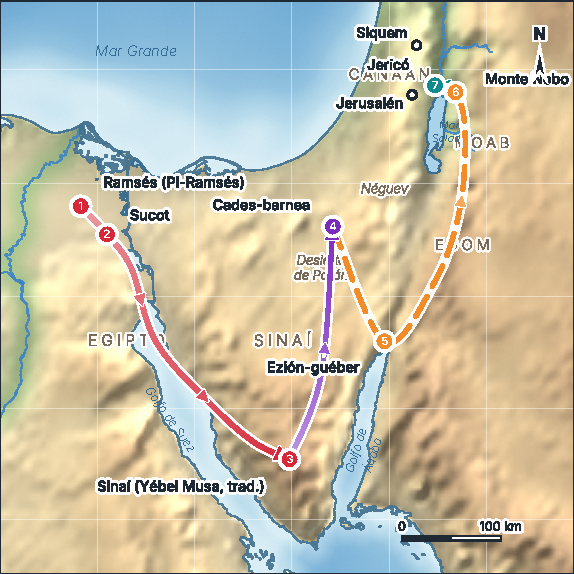
\includegraphics[width=\linewidth,height=0.86\textheight,keepaspectratio]{mapa_exodo.pdf}\par\vspace{1pt}{\fontsize{4.5}{5.5}\selectfont\color{sepia}\textit{Nota.} Elaboración propia (GSHHS/WDB, Basemap); ubicaciones aproximadas.\par}\end{column}
\begin{column}{0.42\textwidth}\scriptsize\RaggedRight
{\scriptsize\RaggedRight
\tikz[baseline=-0.6ex]\draw[ladrillo,line width=1.5pt,line cap=round](0,0)--(0.6,0);~Ruta tradicional: Ramsés $\to$ Sinaí\par
\tikz[baseline=-0.6ex]\draw[cafe,line width=1.5pt,line cap=round](0,0)--(0.6,0);~Sinaí $\to$ Cades (Dt 1:2)\par
\tikz[baseline=-0.6ex]\draw[oro,line width=1.5pt,line cap=round,dash pattern=on 3.4pt off 1.8pt](0,0)--(0.6,0);~Rodeo de Edom $\to$ llanuras de Moab (Nm 20–22)\par}
\medskip

\textbf{Ruta tradicional} (Nm 33): Ramsés, Sucot, el mar, el Sinaí, Cades y el rodeo de Edom hasta las llanuras de Moab.\par\medskip
\textbf{En debate}: el lugar del paso (\heb{יַם־סוּף}, \emph{yam suf}, «mar de los juncos»; LXX «mar Rojo») y el monte Sinaí (Yébel Musa, norte del Sinaí o Madián).\par\medskip
Ein el-Qudeirat (¿Cades?): solo fortalezas del Hierro, aunque un pueblo de tiendas no deja arquitectura.
\end{column}
\end{columns}
\end{frame}

\begin{frame}{Conquista y reparto}
\begin{columns}[c,onlytextwidth]
\begin{column}{0.46\textwidth}\centering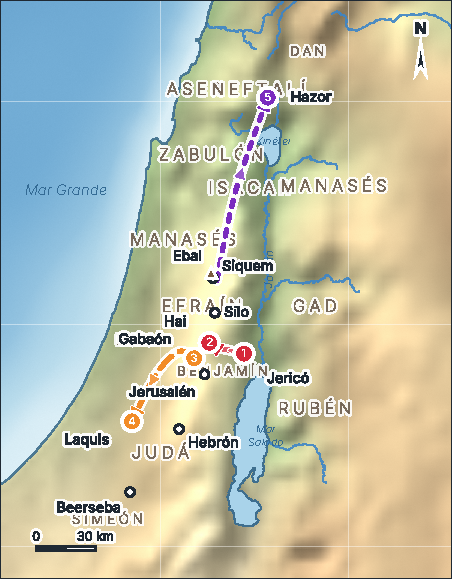
\includegraphics[width=\linewidth,height=0.86\textheight,keepaspectratio]{mapa_tribus.pdf}\par\vspace{1pt}{\fontsize{4.5}{5.5}\selectfont\color{sepia}\textit{Nota.} Elaboración propia (GSHHS/WDB, Basemap); ubicaciones aproximadas.\par}\end{column}
\begin{column}{0.52\textwidth}\scriptsize\RaggedRight
{\scriptsize\RaggedRight
\definecolor{mapacarmesi}{HTML}{D62839}
\definecolor{mapanaranja}{HTML}{F28C28}
\definecolor{mapavioleta}{HTML}{7B2CBF}
\definecolor{mapaturquesa}{HTML}{0F8B8D}
\definecolor{mapaazul}{HTML}{1D4E89}
\definecolor{mapaocre}{HTML}{B5651D}
\tikz[baseline=-0.6ex]{\draw[white,line width=3.2pt,line cap=round](0,0)--(0.62,0);\draw[mapacarmesi,line width=1.8pt,line cap=round,-{Latex[length=1.6mm]}](0,0)--(0.62,0);}~Jericó y Hai (Jos 6–8)\par
\tikz[baseline=-0.6ex]{\draw[white,line width=3.2pt,line cap=round](0,0)--(0.62,0);\draw[mapanaranja,line width=1.8pt,line cap=round,dash pattern=on 3.6pt off 2pt,-{Latex[length=1.6mm]}](0,0)--(0.62,0);}~Gabaón $\to$ sur (Jos 10)\par
\tikz[baseline=-0.6ex]{\draw[white,line width=3.2pt,line cap=round](0,0)--(0.62,0);\draw[mapavioleta,line width=1.8pt,line cap=round,dash pattern=on 1.4pt off 1.6pt,-{Latex[length=1.6mm]}](0,0)--(0.62,0);}~Campaña del norte (Jos 11)\par
\smallskip{\color{black!70}\textbf{Itinerario}}\par
\tikz[baseline=-0.7ex]\node[circle,fill=mapacarmesi,draw=white,line width=0.5pt,text=white,font=\fontsize{5}{5}\selectfont\bfseries,inner sep=0.6pt,minimum size=2.6mm]{1};\,Jericó\quad \tikz[baseline=-0.7ex]\node[circle,fill=mapacarmesi,draw=white,line width=0.5pt,text=white,font=\fontsize{5}{5}\selectfont\bfseries,inner sep=0.6pt,minimum size=2.6mm]{2};\,Hai\quad \tikz[baseline=-0.7ex]\node[circle,fill=mapanaranja,draw=white,line width=0.5pt,text=white,font=\fontsize{5}{5}\selectfont\bfseries,inner sep=0.6pt,minimum size=2.6mm]{3};\,Gabaón\quad \tikz[baseline=-0.7ex]\node[circle,fill=mapanaranja,draw=white,line width=0.5pt,text=white,font=\fontsize{5}{5}\selectfont\bfseries,inner sep=0.6pt,minimum size=2.6mm]{4};\,Laquis\quad \tikz[baseline=-0.7ex]\node[circle,fill=mapavioleta,draw=white,line width=0.5pt,text=white,font=\fontsize{5}{5}\selectfont\bfseries,inner sep=0.6pt,minimum size=2.6mm]{5};\,Hazor\par
\makebox[0.62cm][c]{\tikz[baseline=-0.6ex]\node[circle,fill=white,draw=black!80,line width=0.8pt,inner sep=1.2pt]{};}~Tribus: ubicación aproximada (Jos 13–19)\par}
\medskip

\textbf{Centro} (Jos 6--9): Jericó, Hai y el pacto con Gabaón; Siquem y el Ebal (8:30--35).\par\smallskip
\textbf{Sur} (Jos 10): de Gabaón a Laquis y Hebrón.\par\smallskip
\textbf{Norte} (Jos 11): Hazor, «cabeza de todos aquellos reinos».\par\medskip
\textbf{Reparto} (Jos 13--19): nueve tribus y media al oeste del Jordán; Rubén, Gad y media Manasés al este. Leví no recibe territorio: «YHWH es su heredad» (Jos 13:33).\par\medskip
\precision{los límites tribales se representan con rótulos aproximados.}
\end{column}
\end{columns}
\end{frame}

\begin{frame}{Canaán bajo Egipto}
\centering
\begin{tikzpicture}
 \foreach \x/\n/\t/\d/\r in {0/1/{Cartas de Amarna}/{Ciudades-estado vasallas de Egipto. Abdi-Heba de Jerusalén: los \emph{habiru} saquean las tierras del rey.}/{s. \textsc{xiv} a.\,e.\,c.; EA 286--290; Moran, 1992},
   3.15/2/{¿Habiru = hebreos?}/{No sin más: categoría social (desarraigados, mercenarios), de Mesopotamia a Egipto.}/{\heb{עִבְרִי}: relación en debate},
   6.3/3/{Shasu de \emph{Yhw}}/{Listas de Soleb y Amara West: «tierra de los shasu de \emph{Yhw}», región de Seir (cf. Dt 33:2; Jue 5:4).}/{Lectura discutida},
   9.45/4/{Merneptah}/{«Israel está devastado; su descendencia no existe». Israel con determinativo de pueblo.}/{c. 1208 a.\,e.\,c.}}{
  \node[caja,anchor=north] (b\n) at (\x,0) {\parbox[t][3.35cm][t]{2.65cm}{\RaggedRight
    {\small\textbf{\textcolor{ladrillo}{\t}}}\\[4pt]\scriptsize \d\par\vfill{\tiny\color{sepia}(\r)}}};
  \node[circle,fill=cafe,text=piedra,font=\scriptsize\bfseries,inner sep=1.6pt] at (b\n.north west) {\n};}
\end{tikzpicture}\par\vspace{9pt}
\begin{minipage}{0.95\linewidth}\scriptsize Límite que impone Merneptah: hacia fines del siglo \textsc{xiii}, Israel ya es un pueblo asentado en Canaán.\par
\precision{Deir Alla (s. \textsc{viii}): «Escrito de Balaam, hijo de Beor, el que veía a los dioses» (Hoftijzer y van der Kooij, 1976).}\end{minipage}
\end{frame}

\begin{frame}{La conquista ante la arqueología}
\begin{columns}[t,onlytextwidth]
\begin{column}{0.49\textwidth}\scriptsize\RaggedRight
\begin{itemize}
\item \textbf{Jericó.} Garstang: destrucción c. 1400. Kenyon: c. 1550, casi vacía en el s. \textsc{xiii}. Wood (1990): de nuevo c. 1400. Radiocarbono: s. \textsc{xvi} (Bruins y van der Plicht, 1995).
\item \textbf{Hai} (\heb{הָעַי}, «la ruina»). Et-Tell, sin ciudad en el Bronce Tardío (Callaway, 1968). ¿Etiología, Betel o Khirbet el-Maqatir?
\end{itemize}
\end{column}
\begin{column}{0.49\textwidth}\scriptsize\RaggedRight
\begin{itemize}
\item \textbf{Hazor.} Destrucción por fuego del s. \textsc{xiii}; Ben-Tor: Israel (Jos 11:10--13); otros: revuelta interna (Zuckerman, 2007).
\item \textbf{Monte Ebal.} Zertal: el altar de Jos 8:30--35; Kempinski: torre de vigilancia. La «tablilla de maldición» de 2023 es muy cuestionada.
\item \textbf{Sierra central (Hierro I).} Cientos de aldeas nuevas, casas de cuatro espacios, sin huesos de cerdo (Finkelstein, 1988; Faust, 2006).
\end{itemize}
\end{column}
\end{columns}\vspace{4pt}
\begin{tcolorbox}[colback=piedra,colframe=cafe,boxrule=0.8pt,arc=3pt,fontupper=\scriptsize]
Josué narra la destrucción de solo tres ciudades (Jericó, Hai, Hazor), seguida de un asentamiento largo e incompleto (Jos 13:1; Jue 1).
\end{tcolorbox}
\end{frame}

\begin{frame}{Modelos del origen de Israel}
\centering\scriptsize\renewcommand{\arraystretch}{1.25}
\begin{tabular}{>{\RaggedRight\arraybackslash}p{2.1cm}>{\RaggedRight\arraybackslash}p{2.9cm}>{\RaggedRight\arraybackslash}p{3.3cm}>{\RaggedRight\arraybackslash}p{3.1cm}}
\toprule
\textbf{Modelo} & \textbf{Autores} & \textbf{Propuesta} & \textbf{Dificultad}\\\midrule
Conquista militar & Albright; Yadin; Wood; Kitchen & Una campaña destruye ciudades cananeas & Fechas de Jericó y Hai\\
Infiltración pacífica & Alt (1925); Noth & Pastores se asientan poco a poco & Ignora la memoria de guerra\\
Revuelta campesina & Mendenhall (1962); Gottwald (1979) & Campesinos rompen con las ciudades en torno a YHWH & Poca evidencia directa\\
Surgimiento local & Finkelstein; Dever; Faust & Población local con aportes externos & Choca con la memoria unánime de Egipto\\
\bottomrule
\end{tabular}\par\vspace{6pt}
\begin{minipage}{0.93\linewidth}\precision{el \emph{jérem} (\heb{חֵרֶם}) aparece también en la Estela de Mesa; los relatos antiguos de conquista son hiperbólicos (Younger, 1990); Rahab muestra que no se definía por la etnia.}\end{minipage}
\end{frame}

% ===================================================
\section{El relato}
\begin{frame}{Pascua y paso del mar}
\begin{columns}[t,onlytextwidth]
\begin{column}{0.5\textwidth}
\centering{\large\heb{מִי־כָמֹכָה בָּאֵלִם יְהוָה}}\par\smallskip
\begin{cita}¿Quién como tú entre los dioses, oh YHWH? ¿Quién como tú, magnífico en santidad?\fuente{(Éx 15:11)}\end{cita}
\small \heb{יְהוָה יִמְלֹךְ לְעֹלָם וָעֶד}: «YHWH reinará por siempre jamás» (15:18), primera confesión del reinado de Dios.
\end{column}
\begin{column}{0.48\textwidth}\small\RaggedRight
\begin{itemize}
\item \heb{פָּסַח} (\emph{pasaj}): el destructor «pasa de largo» (Éx 12:13); \heb{זִכָּרוֹן}, memorial perpetuo.
\item Una misma ley para el nativo y el extranjero (12:49).
\item «YHWH peleará por vosotros» (14:14); el pueblo «creyó» (14:31).
\item El cántico ya apunta a la tierra y al santuario (15:13, 17).
\item «Nuestra Pascua, Cristo» (1~Co 5:7); Ap 15:3.
\end{itemize}
\end{column}
\end{columns}
\end{frame}

\begin{frame}{Sobre alas de águila}
\fotolado{panel_ex19.jpg}{Elaboración propia: Éx 19:5--6 en texto hebreo consonántico (BHS).}
\begin{columns}[c,onlytextwidth]
\begin{column}{0.57\textwidth}
\begin{cita}Vosotros visteis lo que hice a los egipcios, y cómo os tomé sobre alas de águila y os he traído a mí. Ahora, pues, si de veras escucháis mi voz y guardáis mi pacto, seréis mi tesoro especial entre todos los pueblos, porque mía es toda la tierra. Y vosotros me seréis un reino de sacerdotes y una nación santa.\fuente{(Éx 19:4--6)}\end{cita}
\scriptsize
\begin{itemize}
\item \textbf{Lo que Dios hizo}: «os he traído \emph{a mí}».
\item \textbf{La condición}: \heb{אִם־שָׁמוֹעַ תִּשְׁמְעוּ}, «si de veras escucháis».
\item \textbf{La identidad}: tesoro, reino de sacerdotes, nación santa.
\end{itemize}
\end{column}
\begin{column}{0.41\textwidth}\end{column}
\end{columns}
\end{frame}

\begin{frame}{Tres palabras del Sinaí}
\centering
\begin{tikzpicture}
 \foreach \x/\n/\t/\h/\d/\r in {0/1/{Segulá}/{סְגֻלָּה}/{Tesoro personal del rey (1~Cr 29:3). «Porque mía es toda la tierra»: elección sin exclusivismo.}/{LXX \grc{λαὸς περιούσιος}},
   4.2/2/{Mamléjet kohaním}/{מַמְלֶכֶת כֹּהֲנִים}/{Israel es ante las naciones lo que el sacerdote es en Israel: acceso, enseñanza, intercesión.}/{LXX \grc{βασίλειον ἱεράτευμα}},
   8.4/3/{Goy qadosh}/{גּוֹי קָדוֹשׁ}/{Una nación entre las naciones, pero apartada. Santidad de pertenencia que genera conducta (Lv 19:2).}/{LXX \grc{ἔθνος ἅγιον}}}{
  \node[caja,anchor=north] (b\n) at (\x,0) {\parbox[t][3.0cm][t]{3.55cm}{\RaggedRight
    {\small\textbf{\textcolor{ladrillo}{\t}}}\hfill\heb{\h}\\[5pt]\scriptsize \d\par\vfill{\scriptsize\color{sepia}\r}}};
  \node[circle,fill=cafe,text=piedra,font=\scriptsize\bfseries,inner sep=1.6pt] at (b\n.north west) {\n};}
\end{tikzpicture}\par\vspace{6pt}
\begin{minipage}{0.92\linewidth}\precision{Sarna (1991) relaciona \emph{segulá} con el acadio \emph{sikiltu} y con un texto de Ugarit donde un rey vasallo es la \emph{sglt} de su señor.}\end{minipage}
\end{frame}

\begin{frame}{Del Sinaí a 1 Pedro}
\centering
\begin{tikzpicture}[node distance=0.9cm]
\node[caja,text width=3.3cm,align=center] (h) {\textbf{Hebreo (Éx 19:6)}\\[3pt]\heb{מַמְלֶכֶת כֹּהֲנִים}\\\heb{וְגוֹי קָדוֹשׁ}};
\node[caja,text width=3.3cm,align=center,right=of h] (g) {\textbf{LXX}\\[3pt]\grc{βασίλειον ἱεράτευμα}\\\grc{καὶ ἔθνος ἅγιον}};
\node[caja,text width=3.3cm,align=center,right=of g] (p) {\textbf{1~P 2:9}\\[3pt]\grc{βασίλειον ἱεράτευμα,}\\\grc{ἔθνος ἅγιον}\\+ Is 43:20--21};
\draw[-{Latex[length=2.5mm]},oro!90!ladrillo,line width=1.4pt] (h) -- (g);
\draw[-{Latex[length=2.5mm]},oro!90!ladrillo,line width=1.4pt] (g) -- (p);
\end{tikzpicture}\par\vspace{8pt}
{\small\itshape\color{sepia}Targum Onqelos: «reyes, sacerdotes»; Ap 1:6 y 5:10: «reino, sacerdotes» (\grc{βασιλείαν, ἱερεῖς}).}\par\vspace{6pt}
\begin{minipage}{0.92\linewidth}\small Pedro escribe a creyentes dispersos, muchos de origen gentil (1~P 1:18; 4:3). Su lectura amplía la vocación de Israel a quienes se unen a ella por el Mesías, como las ramas injertadas de Ro 11:17--24; no la traspasa a otro pueblo.\end{minipage}
\end{frame}

\begin{frame}{El Decálogo y el pacto}
\begin{columns}[t,onlytextwidth]
\begin{column}{0.49\textwidth}
\centering{\heb{אָנֹכִי יְהוָה אֱלֹהֶיךָ אֲשֶׁר הוֹצֵאתִיךָ}}\par\smallskip
\begin{cita}Yo soy YHWH tu Dios, que te saqué de la tierra de Egipto, de casa de esclavos.\fuente{(Éx 20:2)}\end{cita}
\small Primero la gracia, después la obediencia, en el mismo orden que el prólogo histórico de los tratados de vasallaje (Mendenhall, 1954).
\end{column}
\begin{column}{0.49\textwidth}\small\RaggedRight
\begin{itemize}
\item \heb{נַעֲשֶׂה וְנִשְׁמָע}: «haremos y obedeceremos» (Éx 24:7).
\item \heb{הִנֵּה דַם־הַבְּרִית}: «he aquí la sangre del pacto» (24:8); Mt 26:28.
\item Ley como sabiduría «ante los ojos de los pueblos» (Dt 4:6--8).
\item Elegidos no por ser muchos, sino «porque YHWH os amó» y por el juramento a los padres (Dt 7:7--8; Ro 11:28).
\end{itemize}
\end{column}
\end{columns}
\end{frame}

\begin{frame}{Tabernáculo y Shejiná}
\begin{columns}[t,onlytextwidth]
\begin{column}{0.47\textwidth}
\centering{\large\heb{וְעָשׂוּ לִי מִקְדָּשׁ וְשָׁכַנְתִּי בְּתוֹכָם}}\par\smallskip
\begin{cita}Y me harán un santuario, y habitaré en medio de ellos.\fuente{(Éx 25:8)}\end{cita}
\small «La gloria de YHWH llenó el tabernáculo» (Éx 40:34). Pablo: «de ellos es la gloria» (Ro 9:4).
\end{column}
\begin{column}{0.51\textwidth}
\centering
\begin{tikzpicture}[node distance=0.35cm]
\node[caja,text width=1.6cm,align=center] (a1) {\heb{מִשְׁכָּן}\\{\tiny morada}};
\node[caja,text width=1.6cm,align=center,right=of a1] (a2) {\grc{σκηνή}\\{\tiny LXX}};
\node[caja,text width=1.6cm,align=center,right=of a2] (a3) {\grc{ἐσκήνωσεν}\\{\tiny Jn 1:14}};
\node[caja,text width=1.6cm,align=center,below=0.7cm of a1] (b1) {\heb{כַּפֹּרֶת}\\{\tiny tapa del arca}};
\node[caja,text width=1.6cm,align=center,right=of b1] (b2) {\grc{ἱλαστήριον}\\{\tiny LXX Éx 25:17}};
\node[caja,text width=1.6cm,align=center,right=of b2] (b3) {\grc{ἱλαστήριον}\\{\tiny Ro 3:25}};
\foreach \u/\v in {a1/a2,a2/a3,b1/b2,b2/b3}{\draw[-{Latex[length=2mm]},oro!90!ladrillo,line width=1.2pt] (\u) -- (\v);}
\end{tikzpicture}\par\vspace{6pt}
{\scriptsize\itshape\color{sepia}\emph{Shajan}, «habitar en tienda», da nombre al \emph{mishkán} y al término rabínico \emph{Shejiná}.}
\end{column}
\end{columns}
\end{frame}

\begin{frame}{Un sacerdocio en círculos}
\begin{columns}[c,onlytextwidth]
\begin{column}{0.46\textwidth}
\centering
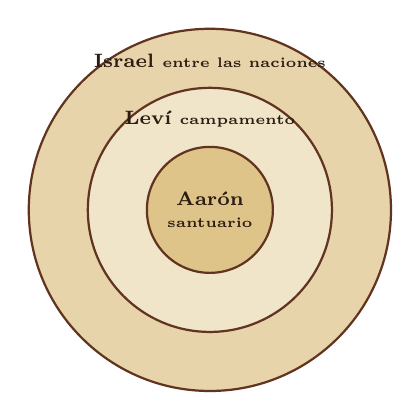
\begin{tikzpicture}
\fill[piedra!80!oro,draw=cafe,line width=0.8pt] (0,0) circle (2.3);
\fill[oro!25,draw=cafe,line width=0.8pt] (0,0) circle (1.55);
\fill[oro!55,draw=cafe,line width=0.8pt] (0,0) circle (0.8);
\node[font=\scriptsize\bfseries,text=tinta,align=center] at (0,0) {Aarón\\{\tiny santuario}};
\node[font=\scriptsize\bfseries,text=tinta,align=center] at (0,1.15) {Leví {\tiny campamento}};
\node[font=\scriptsize\bfseries,text=tinta,align=center] at (0,1.9) {Israel {\tiny entre las naciones}};
\end{tikzpicture}
\end{column}
\begin{column}{0.52\textwidth}
\begin{cita}He tomado a los levitas [\ldots] en lugar de todos los primogénitos, porque mío es todo primogénito.\fuente{(Nm 3:12--13)}\end{cita}
\scriptsize
\begin{itemize}
\item Israel, primogénito entre las naciones (Éx 4:22); sus primogénitos, librados en la Pascua y representados por los levitas.
\item Bendición sacerdotal: «pondrán mi nombre sobre los hijos de Israel» (Nm 6:24--27).
\item Ketef Hinom (fines s. \textsc{vii}--inicios s. \textsc{vi} a.\,e.\,c.): dos rollitos de plata con esta bendición, los textos bíblicos más antiguos conservados (Barkay et al., 2004).
\end{itemize}
\end{column}
\end{columns}
\end{frame}

\begin{frame}{El becerro de oro}
\begin{columns}[t,onlytextwidth]
\begin{column}{0.49\textwidth}\small\RaggedRight
\begin{itemize}
\item Al pie del monte, cuarenta días después de «haremos y obedeceremos» (Éx 32:1--6).
\item Dios propone empezar de nuevo con Moisés (32:10).
\item Moisés intercede: es tu pueblo; tu nombre ante Egipto; «acuérdate de Abraham, de Isaac y de Israel» (32:11--13).
\item «Si no, ráeme de tu libro» (32:32).
\end{itemize}
\end{column}
\begin{column}{0.49\textwidth}
\begin{cita}Desearía yo mismo ser anatema, separado del Mesías, por amor a mis hermanos.\fuente{(Ro 9:3)}\end{cita}
\centering{\footnotesize\grc{ηὐχόμην γὰρ ἀνάθεμα εἶναι αὐτὸς ἐγώ}}\par\smallskip
\small Romanos 9--11 se abre con una intercesión de tono mosaico (Moo, 1996).
\end{column}
\end{columns}
\end{frame}

\begin{frame}{El nombre misericordioso}
\fotolado{panel_ex34.jpg}{Elaboración propia: Éx 34:6--7 en texto hebreo consonántico (BHS).}
\begin{columns}[c,onlytextwidth]
\begin{column}{0.57\textwidth}
\begin{cita}¡YHWH, YHWH, Dios compasivo y clemente, lento para la ira y grande en misericordia y fidelidad; que guarda misericordia a millares, que perdona la iniquidad, la rebelión y el pecado!\fuente{(Éx 34:6--7)}\end{cita}
\scriptsize
\begin{itemize}
\item Se revela \textbf{después} de que Israel rompe el pacto.
\item \heb{חֶסֶד} (\emph{jésed}) y \heb{אֱמֶת} (\emph{emet}); \heb{רַחוּם}, de \heb{רֶחֶם}, «seno materno».
\item Citado en Nm 14:18; Sal 86:15; 103:8; Jl 2:13; Jon 4:2; Neh 9:17.
\item Dios renueva el pacto y escribe de nuevo las tablas (Éx 34:1, 10).
\end{itemize}
\end{column}
\begin{column}{0.41\textwidth}\end{column}
\end{columns}
\end{frame}

\begin{frame}{Cades: perdón y remanente}
\begin{columns}[c,onlytextwidth]
\begin{column}{0.49\textwidth}\small\RaggedRight
\begin{itemize}
\item El pueblo propone volver a Egipto, es decir, deshacer el Éxodo (Nm 14:4).
\item Moisés cita Éx 34:6--7 (Nm 14:17--19).
\item \heb{סָלַחְתִּי כִּדְבָרֶךָ}: «lo he perdonado conforme a tu palabra» (14:20).
\item Pero la generación incrédula muere en el desierto; sus hijos entran (14:22--31).
\end{itemize}
\end{column}
\begin{column}{0.49\textwidth}
\centering
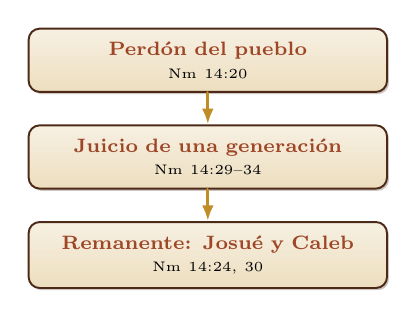
\begin{tikzpicture}[node distance=0.4cm]
\node[caja,text width=4.2cm,align=center] (a) {\textbf{\textcolor{ladrillo}{Perdón del pueblo}}\\{\tiny Nm 14:20}};
\node[caja,text width=4.2cm,align=center,below=of a] (b) {\textbf{\textcolor{ladrillo}{Juicio de una generación}}\\{\tiny Nm 14:29--34}};
\node[caja,text width=4.2cm,align=center,below=of b] (c) {\textbf{\textcolor{ladrillo}{Remanente: Josué y Caleb}}\\{\tiny Nm 14:24, 30}};
\draw[-{Latex[length=2mm]},oro!90!ladrillo,line width=1.2pt] (a) -- (b);
\draw[-{Latex[length=2mm]},oro!90!ladrillo,line width=1.2pt] (b) -- (c);
\end{tikzpicture}\par\smallskip
{\scriptsize\itshape\color{sepia}La secuencia que Pablo reconoce en Ro 11:5: «un remanente escogido por gracia».}
\end{column}
\end{columns}
\end{frame}

\begin{frame}{Balaam y Baal-peor}
\begin{columns}[t,onlytextwidth]
\begin{column}{0.52\textwidth}
\centering{\heb{הֶן־עָם לְבָדָד יִשְׁכֹּן}}\par\smallskip
\begin{cita}He aquí un pueblo que habitará solo, y no será contado entre las naciones.\fuente{(Nm 23:9)}\end{cita}
\centering{\heb{דָּרַךְ כּוֹכָב מִיַּעֲקֹב}}\par\smallskip
\begin{cita}Saldrá una estrella de Jacob, y se levantará un cetro de Israel.\fuente{(Nm 24:17)}\end{cita}
\end{column}
\begin{column}{0.46\textwidth}\scriptsize\RaggedRight
\begin{itemize}
\item Targum Onqelos: «se levantará un rey de Jacob y será ungido el Mesías de Israel».
\item Qumrán: CD \textsc{vii} 18--21; 4Q175. Rabí Aquiba y Bar Kojba, «hijo de la estrella» (TJ Taanit 4:5).
\item Baal-peor (Nm 25), por consejo de Balaam (Nm 31:16; Ap 2:14); Finees y el «pacto de sacerdocio perpetuo».
\end{itemize}
\precision{la \emph{Octava lección} sitúa en Balaam la entrada de la idolatría. El episodio pesa (Os 9:10), pero el becerro (Éx 32) es anterior, y Jos 24:14 y Ez 20:7--8 la remontan a Egipto.}
\end{column}
\end{columns}
\end{frame}

\begin{frame}{Deuteronomio en Moab}
\begin{columns}[t,onlytextwidth]
\begin{column}{0.49\textwidth}
\centering{\large\heb{שְׁמַע יִשְׂרָאֵל יְהוָה אֱלֹהֵינוּ יְהוָה אֶחָד}}\par\smallskip
\begin{cita}Escucha, Israel: YHWH nuestro Dios, YHWH uno es. Y amarás a YHWH tu Dios con todo tu corazón.\fuente{(Dt 6:4--5)}\end{cita}
\end{column}
\begin{column}{0.49\textwidth}\small
\begin{itemize}
\item La Torá predicada a la generación nacida en el desierto.
\item Renovación del pacto: bendiciones y maldiciones (Dt 27--30).
\item El Cántico de Moisés como testigo (Dt 31:19; 32).
\item «Profeta como yo te levantará YHWH» (Dt 18:15; Hch 3:22).
\item «Nunca más se levantó profeta como Moisés» (Dt 34:10).
\end{itemize}
\end{column}
\end{columns}
\end{frame}

\begin{frame}{Josué: la entrada en la tierra}
\centering
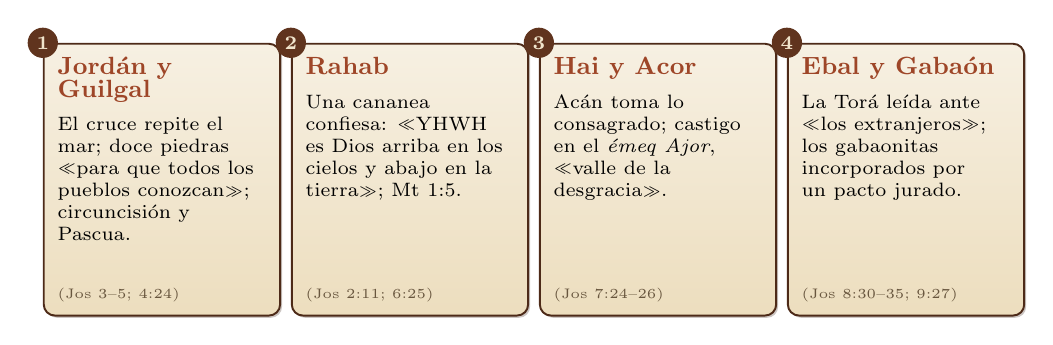
\begin{tikzpicture}
 \foreach \x/\n/\t/\d/\r in {0/1/{Jordán y Guilgal}/{El cruce repite el mar; doce piedras «para que todos los pueblos conozcan»; circuncisión y Pascua.}/{Jos 3--5; 4:24},
   3.15/2/{Rahab}/{Una cananea confiesa: «YHWH es Dios arriba en los cielos y abajo en la tierra»; Mt 1:5.}/{Jos 2:11; 6:25},
   6.3/3/{Hai y Acor}/{Acán toma lo consagrado; castigo en el \emph{émeq Ajor}, «valle de la desgracia».}/{Jos 7:24--26},
   9.45/4/{Ebal y Gabaón}/{La Torá leída ante «los extranjeros»; los gabaonitas incorporados por un pacto jurado.}/{Jos 8:30--35; 9:27}}{
  \node[caja,anchor=north] (b\n) at (\x,0) {\parbox[t][3.1cm][t]{2.65cm}{\RaggedRight
    {\small\textbf{\textcolor{ladrillo}{\t}}}\\[4pt]\scriptsize \d\par\vfill{\tiny\color{sepia}(\r)}}};
  \node[circle,fill=cafe,text=piedra,font=\scriptsize\bfseries,inner sep=1.6pt] at (b\n.north west) {\n};}
\end{tikzpicture}\par\vspace{5pt}
\begin{minipage}{0.95\linewidth}\scriptsize \heb{יְהוֹשֻׁעַ} (\emph{Yehoshúa}, «YHWH salva»), en griego \grc{Ἰησοῦς}: «si Josué les hubiera dado el reposo\ldots» (Heb 4:8).\end{minipage}
\end{frame}

\begin{frame}{La tierra dada, el pacto renovado}
\begin{columns}[t,onlytextwidth]
\begin{column}{0.49\textwidth}
\begin{cita}No faltó palabra de todas las buenas promesas que YHWH había hecho a la casa de Israel; todo se cumplió.\fuente{(Jos 21:45)}\end{cita}
\small \heb{נַחֲלָה} (\emph{najalá}): heredad que no se vende a perpetuidad, «porque la tierra mía es» (Lv 25:23). Aun así, «queda mucha tierra por poseer» (Jos 13:1).\par\smallskip
\precision{el Códice de Leningrado omite Jos 21:36--37; algunas ediciones hebreas numeran 21:41--43.}
\end{column}
\begin{column}{0.49\textwidth}
\centering{\heb{וְאָנֹכִי וּבֵיתִי נַעֲבֹד אֶת־יְהוָה}}\par\smallskip
\begin{cita}Pero yo y mi casa serviremos a YHWH.\fuente{(Jos 24:15)}\end{cita}
\small Siquem: donde Abraham recibió la promesa (Gn 12:6--7). Renovación del pacto; los huesos de José sepultados allí (Jos 24:32; Gn 50:25).
\end{column}
\end{columns}
\end{frame}

% ===================================================
\section{Vocación}
\begin{frame}{Vivida, quebrada, preservada}
\centering\scriptsize\renewcommand{\arraystretch}{1.25}
\begin{tabular}{>{\RaggedRight\arraybackslash}p{3.6cm}>{\RaggedRight\arraybackslash}p{3.4cm}>{\RaggedRight\arraybackslash}p{4.0cm}}
\toprule
\textbf{Se vivió} & \textbf{Se quebró} & \textbf{Se preservó}\\\midrule
«Haremos y obedeceremos» (Éx 24:7) & Becerro de oro (Éx 32) & Intercesión; nombre misericordioso (Éx 34:6--7)\\
La gloria en el tabernáculo (Éx 40:34) & Rebelión de Cades (Nm 14) & Perdón; remanente: Josué y Caleb\\
Torá ante extranjeros; Rahab; Gabaón (Jos 8:35) & Baal-peor (Nm 25) & Finees: «sacerdocio perpetuo» (Nm 25:13)\\
Levitas fieles (Éx 32:26--29) & Acán (Jos 7) & Pacto renovado en Ebal y Siquem\\
\bottomrule
\end{tabular}\par\vspace{8pt}
\begin{minipage}{0.93\linewidth}\small
\destacar{Hacia las naciones} desde el comienzo (Éx 12:49; Dt 4:6). \destacar{Santidad por presencia}: «¿en qué se conocerá\ldots sino en que tú andes con nosotros?» (Éx 33:16). \destacar{Mediador y remanente} cuando el pueblo falla.
\end{minipage}
\end{frame}

% ===================================================
\section{Tradición judía}
\begin{frame}{Shavuot y la Torá para todos}
\begin{columns}[t,onlytextwidth]
\begin{column}{0.49\textwidth}\small
\textbf{\textcolor{ladrillo}{Shavuot}}\par\smallskip
Fiesta de primicias (Lv 23:15--21); unida al Sinaí por Éx 19:1. Los Diez Mandamientos, el 6 de Siván según los sabios, el 7 según rabí Yosé (Shabat 86b). Liturgia: \heb{זְמַן מַתַּן תּוֹרָתֵנוּ}.\par\smallskip
«Cada palabra se dividía en setenta lenguas» (Shabat 88b). Posible eco en Hch 2, aunque no demostrado.
\end{column}
\begin{column}{0.49\textwidth}\small
\textbf{\textcolor{ladrillo}{La Torá ofrecida a las naciones}}\par\smallskip
Sobre Dt 33:2: antes que a Israel, Dios ofreció la Torá a Esaú, a Amón y Moab y a Ismael, que la rehusaron (Sifré Deuteronomio 343).\par\smallskip
Se dio en el desierto, lugar sin dueño, para que ninguna nación dijera que no tenía parte en ella (Mekhilta, Bajódesh 5).\par\smallskip
{\itshape\color{sepia}Cf. Éx 19:5: «mía es toda la tierra».}
\end{column}
\end{columns}
\end{frame}

\begin{frame}{El calendario de la memoria}
\begin{columns}[t,onlytextwidth]
\begin{column}{0.32\textwidth}\small
\textbf{\textcolor{ladrillo}{17 de Tamuz y Yom Kipur}}\par\smallskip
Se rompen las tablas el 17 de Tamuz (Mishná, Taanit 4:6); las segundas, el 10 de Tishré (Seder Olam 6; Rashi). Las \emph{trece midot} de Éx 34:6--7, «orden de la plegaria» para el perdón (Rosh Hashaná 17b).
\end{column}
\begin{column}{0.33\textwidth}\small
\textbf{\textcolor{ladrillo}{9 de Av}}\par\smallskip
«Se decretó contra nuestros padres que no entrarían en la tierra»; en esa fecha cayeron ambos templos (Taanit 4:6). «Llorasteis por nada; os estableceré un llanto por generaciones» (Taanit 29a).
\end{column}
\begin{column}{0.32\textwidth}\small
\textbf{\textcolor{ladrillo}{Pésaj y Sukkot}}\par\smallskip
\emph{Az yashir} y \emph{Mi jamoja} cada mañana; \emph{Dayenu} en el Séder. Cabañas: nubes de gloria (R. Eliézer) o cabañas reales (R. Aquiba) (Sukká 11b); Zac 14:16.
\end{column}
\end{columns}
\end{frame}

\begin{frame}{La cadena de la tradición}
\centering{\large\heb{משה קבל תורה מסיני ומסרה ליהושע}}\par\smallskip
\begin{cita}Moisés recibió la Torá desde el Sinaí y la transmitió a Josué; Josué, a los ancianos; los ancianos, a los profetas.\fuente{(Mishná, Avot 1:1)}\end{cita}
\begin{columns}[t,onlytextwidth]
\begin{column}{0.49\textwidth}\scriptsize
\begin{itemize}
\item Josué escribió su libro y los ocho versículos finales de la Torá (Bava Batra 15a).
\item Rahab, esposa de Josué y antepasada de profetas, entre ellos Jeremías (Meguilá 14b): haggadá.
\end{itemize}
\end{column}
\begin{column}{0.49\textwidth}\scriptsize
\begin{itemize}
\item Las manos de Moisés: «mientras Israel miraba hacia arriba [\ldots] prevalecía» (Mishná, Rosh Hashaná 3:8).
\item Josefo: tabernáculo como imagen del cosmos (\emph{Ant.} 3.7.7); muerte de Moisés (\emph{Ant.} 4.8.48).
\end{itemize}
\end{column}
\end{columns}
\end{frame}

% ===================================================
\section{Restauración}
\begin{frame}{La promesa en la Torá}
\centering\scriptsize\renewcommand{\arraystretch}{1.22}
\begin{tabular}{>{\RaggedRight\arraybackslash}p{2.1cm}>{\RaggedRight\arraybackslash}p{4.6cm}>{\RaggedRight\arraybackslash}p{4.4cm}}
\toprule
\textbf{Texto} & \textbf{Promesa} & \textbf{Proyección}\\\midrule
Éx 32:13; 34:6--10 & Perdón por el juramento a los padres y el nombre misericordioso & Jl 2:13; Jon 4:2; Sal 103:8\\
Nm 14:20--24 & Perdón, juicio de una generación, remanente & Is 10:20--22; Ro 11:5\\
Nm 24:17 & Estrella de Jacob & 4Q175; Mt 2:2\\
Dt 4:25--31 & Destierro y regreso «en los postreros días» & Os 3:5; Jer 29:12--14\\
Dt 30:1--10 & Regreso; corazón circuncidado & Jer 31:33 [31:32]; Ez 36:26; Ro 10:6--8\\
Dt 32:21, 43 & Celos; las naciones con su pueblo & Ro 10:19; 11:11; 15:10\\
\bottomrule
\end{tabular}\par\vspace{6pt}
\centering{\heb{כִּי אֵל רַחוּם יְהוָה אֱלֹהֶיךָ}}\par\smallskip
\begin{cita}[fontupper=\scriptsize\itshape]En los postreros días volverás a YHWH tu Dios [\ldots]. Porque Dios compasivo es YHWH tu Dios; no te dejará [\ldots] ni se olvidará del pacto que juró a tus padres.\fuente{(Dt 4:30--31)}\end{cita}
\end{frame}

\begin{frame}{El corazón circuncidado}
\fotolado{panel_dt30.jpg}{Elaboración propia: Dt 30:6 en texto hebreo consonántico (BHS).}
\begin{columns}[c,onlytextwidth]
\begin{column}{0.57\textwidth}
\begin{cita}Y circuncidará YHWH tu Dios tu corazón y el corazón de tu descendencia, para que ames a YHWH tu Dios con todo tu corazón y con toda tu alma, a fin de que vivas.\fuente{(Dt 30:6)}\end{cita}
\scriptsize
\begin{itemize}
\item Israel «volverá» (\emph{shuv}); Dios «hará volver tu cautividad» (\heb{אֶת־שְׁבוּתְךָ}, 30:3) y lo recogerá «del extremo de los cielos» (30:4).
\item Dt 10:16: mandato; Dt 30:6: promesa. Dios mismo hace posible el Shemá.
\item Jeremías: «nuevo pacto»; Ezequiel: «corazón nuevo» (Ez 36:26--27).
\item ONE FOR ISRAEL (2025) incluye Dt 4:30--31 entre los textos del regreso nacional esperado en Ro 11:26.
\end{itemize}
\end{column}
\begin{column}{0.41\textwidth}\end{column}
\end{columns}
\end{frame}

\begin{frame}{El Cántico de Moisés}
\begin{columns}[t,onlytextwidth]
\begin{column}{0.49\textwidth}\small
Elección (32:8--9), cuidado «como el águila» (32:11), infidelidad, juicio y compasión: «por amor de sus siervos se arrepentirá» (32:36).\par\medskip
\precision{Dt 32:8: TM «hijos de Israel»; 4QDeut\textsuperscript{j} «hijos de Dios»; LXX «ángeles de Dios». Dt 32:43: 4QDeut\textsuperscript{q} y LXX más largos (Tov, 2012).}
\end{column}
\begin{column}{0.49\textwidth}
\centering\scriptsize\renewcommand{\arraystretch}{1.2}
\begin{tabular}{>{\RaggedRight\arraybackslash}p{1.1cm}>{\RaggedRight\arraybackslash}p{4.4cm}}
\toprule
\multicolumn{2}{l}{\textbf{Dt 32:21}}\\\midrule
TM & \heb{וַאֲנִי אַקְנִיאֵם בְּלֹא־עָם}\\
LXX & \grc{κἀγὼ παραζηλώσω αὐτοὺς ἐπ᾽ οὐκ ἔθνει}\\
Ro 10:19 & \grc{ἐγὼ παραζηλώσω ὑμᾶς ἐπ᾽ οὐκ ἔθνει}\\\midrule
\multicolumn{2}{l}{\textbf{Dt 32:43}}\\\midrule
TM & \heb{הַרְנִינוּ גוֹיִם עַמּוֹ}\\
LXX = Ro 15:10 & \grc{εὐφράνθητε, ἔθνη, μετὰ τοῦ λαοῦ αὐτοῦ}\\
\bottomrule
\end{tabular}
\end{column}
\end{columns}
\end{frame}

\begin{frame}{Isaías: el nuevo éxodo}
\begin{columns}[t,onlytextwidth]
\begin{column}{0.5\textwidth}
\centering{\heb{אַיֵּה הַשָּׂם בְּקִרְבּוֹ אֶת־רוּחַ קָדְשׁוֹ}}\par\smallskip
\begin{cita}¿Dónde el que los hizo subir del mar con el pastor de su rebaño? ¿Dónde el que puso en medio de él su Santo Espíritu? [\ldots] El Espíritu de YHWH los hizo descansar.\fuente{(Is 63:11, 14)}\end{cita}
\end{column}
\begin{column}{0.48\textwidth}\scriptsize\RaggedRight
\begin{itemize}
\item \textbf{Is 63:7--14}: el Éxodo releído como obra del Espíritu; el recuerdo hecho oración (63:16).
\item \textbf{Is 43:16--21}: el Dios «que abre camino en el mar»; \heb{עַם־זוּ יָצַרְתִּי לִי}, «este pueblo he formado para mí» (cf. 1~P 2:9).
\item \textbf{Is 11:16}: camino para el remanente «como el día que subió de Egipto».
\item \textbf{Is 61:6}: «seréis llamados sacerdotes de YHWH»: Éx 19:6 cumplido.
\end{itemize}
\end{column}
\end{columns}
\end{frame}

\begin{frame}{Jeremías: el nuevo pacto}
\begin{columns}[t,onlytextwidth]
\begin{column}{0.53\textwidth}
\begin{cita}[fontupper=\scriptsize\itshape]Haré un nuevo pacto con la casa de Israel y con la casa de Judá. No como el pacto que hice con sus padres el día que los tomé de la mano para sacarlos de la tierra de Egipto [\ldots]. Pondré mi ley en su interior y la escribiré en su corazón.\fuente{(Jer 31:31--33 [31:30--32])}\end{cita}
\scriptsize La ley es la misma; cambia el lugar donde se escribe (Dt 30:6). Destinatarios: casa de Israel (norte) y casa de Judá (sur).
\end{column}
\begin{column}{0.45\textwidth}\scriptsize
\begin{itemize}
\item \textbf{Jer 2:2--3}: el desierto como noviazgo; «santo era Israel para YHWH, primicias de sus frutos» (cf. Ro 11:16).
\item \textbf{Jer 7:22--23}: en el Éxodo Dios no habló primero de sacrificios, sino de «escuchad mi voz» (Éx 19:5).
\item \textbf{Ro 11:27}: «este será mi pacto con ellos, cuando yo quite sus pecados».
\end{itemize}
\end{column}
\end{columns}
\end{frame}

\begin{frame}{Oseas: puerta de esperanza}
\centering{\large\heb{וְאֶת־עֵמֶק עָכוֹר לְפֶתַח תִּקְוָה}}\par\smallskip
\begin{cita}La llevaré al desierto y le hablaré al corazón [\ldots], y el valle de Acor por puerta de esperanza; y allí responderá como en el día en que subió de la tierra de Egipto.\fuente{(Os 2:14--15 [2:16--17])}\end{cita}
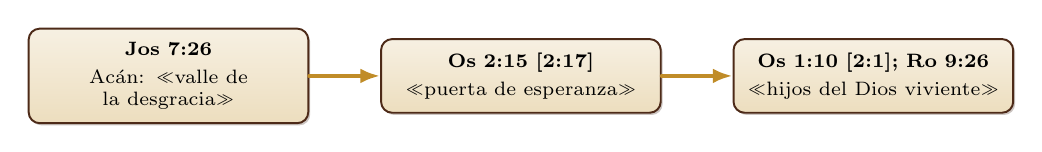
\begin{tikzpicture}[node distance=0.9cm]
\node[caja,text width=3.2cm,align=center] (a) {\textbf{Jos 7:26}\\[2pt]Acán: «valle de la desgracia»};
\node[caja,text width=3.2cm,align=center,right=of a] (b) {\textbf{Os 2:15 [2:17]}\\[2pt]«puerta de esperanza»};
\node[caja,text width=3.2cm,align=center,right=of b] (c) {\textbf{Os 1:10 [2:1]; Ro 9:26}\\[2pt]«hijos del Dios viviente»};
\draw[-{Latex[length=2.5mm]},oro!90!ladrillo,line width=1.4pt] (a) -- (b);
\draw[-{Latex[length=2.5mm]},oro!90!ladrillo,line width=1.4pt] (b) -- (c);
\end{tikzpicture}
\end{frame}

\begin{frame}{Pablo lee esta etapa}
\fotolado{panel_1p29.jpg}{Elaboración propia: 1~P 2:9 en escritura uncial (texto NA28).}
\begin{columns}[c,onlytextwidth]
\begin{column}{0.57\textwidth}\scriptsize
\begin{itemize}
\item \textbf{Ro 10:6--8} (Dt 30:12--14): «cerca de ti está la palabra», aplicada a la palabra de fe (cf. Baruc 3:29--30; Targum Neofiti).
\item \textbf{Ro 11:8} (Dt 29:4 [29:3]): ojos que no ven «hasta el día de hoy»; el mismo arco de Dt 29--30: ceguera presente, corazón circuncidado prometido.
\item \textbf{Ro 10:19; 11:11} (Dt 32:21): los celos como medio para atraer de nuevo a Israel.
\item \textbf{Ro 15:10} (Dt 32:43 LXX): «alegraos, naciones, con su pueblo».
\item \textbf{1~Co 10:1--11}: a gentiles, «nuestros padres pasaron el mar» (Hays, 1989).
\end{itemize}
\end{column}
\begin{column}{0.41\textwidth}\end{column}
\end{columns}
\end{frame}

% ===================================================
\section{Síntesis}
\begin{frame}{Síntesis}
\begin{tcolorbox}[colback=piedra,colframe=ladrillo,boxrule=1pt,arc=3pt,fontupper=\small]
\textbf{\textcolor{cafe}{Israel en el Sinaí:}} un pueblo redimido antes de recibir la ley, llamado a ser \emph{segulá}, reino de sacerdotes y nación santa, con Dios habitando en medio de él. Rompe el pacto al pie del monte y en el desierto; Dios responde con su nombre misericordioso, preserva un remanente y anuncia destierro y regreso con un corazón circuncidado (Dt 4; 30). Desde ese horizonte escribe Pablo Romanos 9--11.
\end{tcolorbox}
\scriptsize\renewcommand{\arraystretch}{1.2}
\begin{tabular}{>{\RaggedRight\arraybackslash}p{3.0cm}>{\RaggedRight\arraybackslash}p{8.3cm}}
\toprule
\textbf{Eje} & \textbf{Lo que deja esta etapa}\\\midrule
Redención y vocación & Pascua, mar, Éx 19:4--6; Torá ante los pueblos (Dt 4:6)\\
Presencia y sacerdocio & Tabernáculo y Shejiná; Aarón, Leví, Israel entre las naciones\\
Restauración & Éx 34:6--7; Nm 14:20; Dt 4:25--31; 30:1--10; 32:36--43\\
Proyección & Isaías (nuevo éxodo, Espíritu), Jeremías (nuevo pacto), Oseas (Acor), Pablo (Ro 10--11)\\
\bottomrule
\end{tabular}
\end{frame}

\begin{frame}{Hacia el Estudio 3}
\begin{columns}[c,onlytextwidth]
\begin{column}{0.55\textwidth}
\begin{cita}Se levantó después de ellos otra generación que no conocía a YHWH, ni la obra que él había hecho por Israel.\fuente{(Jue 2:10)}\end{cita}
\small La tierra fue dada (Jos 21:45), pero la generación siguiente olvidará el Éxodo y entrará en un ciclo de \destacar{apostasía}, \destacar{opresión}, \destacar{clamor} y \destacar{liberación}.
\end{column}
\begin{column}{0.42\textwidth}
\begin{tcolorbox}[colback=cafe,colframe=cafeosc,coltext=piedra,boxrule=0.8pt,arc=3pt,fontupper=\small]
\textbf{Estudio 3}\par\smallskip
De los Jueces a David: ciclos de apostasía y liberación, Rut la moabita, Samuel, Saúl y la unción de David.
\end{tcolorbox}
\end{column}
\end{columns}
\end{frame}

% ===================================================
\section{Reflexión}
\begin{frame}{Para la reflexión}
\small
\begin{enumerate}
\item Dios dice «os he traído a mí» (Éx 19:4) antes de dar mandamiento alguno. ¿Qué cambia al leer la ley desde la redención?
\item Israel es \emph{segulá} de un Dios que dice «mía es toda la tierra». ¿Cómo evita esta frase que la elección se lea como desprecio de las naciones?
\item El nombre misericordioso (Éx 34:6--7) se revela tras el becerro. ¿Qué enseña sobre el pecado de Israel y la fidelidad de Dios en Romanos 11?
\item Pablo dice a gentiles que «nuestros padres» pasaron el mar (1~Co 10:1). ¿Qué responsabilidad trae recibir esa historia (Ro 11:18--21)?
\item ¿Qué dicen Rahab y los gabaonitas sobre el lugar de los gentiles en el pueblo de Dios?
\end{enumerate}
\end{frame}

% ===================================================
\section{Glosario}
\begin{frame}{Glosario}
\begin{columns}[t,onlytextwidth]
\begin{column}{0.49\textwidth}\scriptsize
\textbf{Émeq Ajor} (\heb{עֵמֶק עָכוֹר}): valle de la desgracia; puerta de esperanza (Os 2:15).\par\smallskip
\textbf{Hilastérion} (\grc{ἱλαστήριον}): \emph{kapóret} en la LXX; Ro 3:25.\par\smallskip
\textbf{Jérem} (\heb{חֵרֶם}): consagración al exterminio (Jos 6:17).\par\smallskip
\textbf{Jésed} (\heb{חֶסֶד}): lealtad amorosa del pacto (Éx 34:6).\par\smallskip
\textbf{Kapóret} (\heb{כַּפֹּרֶת}): tapa del arca (Éx 25:17).\par\smallskip
\textbf{Mamléjet kohaním} (\heb{מַמְלֶכֶת כֹּהֲנִים}): reino de sacerdotes.\par\smallskip
\textbf{Mishkán} (\heb{מִשְׁכָּן}): tabernáculo, morada.
\end{column}
\begin{column}{0.49\textwidth}\scriptsize
\textbf{Najalá} (\heb{נַחֲלָה}): heredad (Jos 13--21).\par\smallskip
\textbf{Segulá} (\heb{סְגֻלָּה}): tesoro personal (Éx 19:5).\par\smallskip
\textbf{Shavuot} (\heb{שָׁבוּעוֹת}): fiesta de las Semanas; Pentecostés.\par\smallskip
\textbf{Shelosh esré midot} (\heb{שְׁלֹשׁ עֶשְׂרֵה מִדּוֹת}): trece atributos.\par\smallskip
\textbf{Sukkot} (\heb{סֻכּוֹת}): fiesta de las Cabañas (Lv 23:43).\par\smallskip
\textbf{Yam suf} (\heb{יַם־סוּף}): mar de los juncos.\par\smallskip
\textbf{Yehoshúa} (\heb{יְהוֹשֻׁעַ}): Josué; \grc{Ἰησοῦς}.
\end{column}
\end{columns}
\end{frame}

% ===================================================
\section{Referencias}
\begin{frame}[allowframebreaks]{Referencias}
\tiny
\refapa{Barkay, G., Vaughn, A.~G., Lundberg, M.~J., \& Zuckerman, B. (2004). The amulets from Ketef Hinnom: A new edition and evaluation. \emph{Bulletin of the American Schools of Oriental Research, 334}, 41--71.}
\refapa{\emph{Biblia Hebraica Stuttgartensia} (5.ª ed.). (1997). Deutsche Bibelgesellschaft.}
\refapa{Bimson, J.~J. (1978). \emph{Redating the Exodus and conquest}. JSOT Press.}
\refapa{Bruins, H.~J., \& van der Plicht, J. (1995). Tell es-Sultan (Jericho): Radiocarbon results of short-lived cereal and multiyear charcoal samples from the end of the Middle Bronze Age. \emph{Radiocarbon, 37}(2), 213--220.}
\refapa{Callaway, J.~A. (1968). New evidence on the conquest of `Ai. \emph{Journal of Biblical Literature, 87}(3), 312--320.}
\refapa{Danby, H. (Trad.). (1933). \emph{The Mishnah}. Oxford University Press.}
\refapa{Epstein, I. (Ed.). (1935--1948). \emph{The Babylonian Talmud}. Soncino Press.}
\refapa{Faust, A. (2006). \emph{Israel's ethnogenesis: Settlement, interaction, expansion and resistance}. Equinox.}
\refapa{Finkelstein, I. (1988). \emph{The archaeology of the Israelite settlement}. Israel Exploration Society.}
\refapa{Gottwald, N.~K. (1979). \emph{The tribes of Yahweh}. Orbis Books.}
\refapa{Guggenheimer, H.~W. (1998). \emph{Seder Olam: The rabbinic view of biblical chronology}. Jason Aronson.}
\refapa{Hammer, R. (Trad.). (1986). \emph{Sifre: A Tannaitic commentary on the book of Deuteronomy}. Yale University Press.}
\refapa{Hays, R.~B. (1989). \emph{Echoes of Scripture in the letters of Paul}. Yale University Press.}
\refapa{Hoffmeier, J.~K. (2005). \emph{Ancient Israel in Sinai}. Oxford University Press.}
\refapa{Hoftijzer, J., \& van der Kooij, G. (1976). \emph{Aramaic texts from Deir `Alla}. Brill.}
\refapa{\emph{Israel, el pueblo de Dios} (Octava lección) [Material de estudio congregacional]. (s.\,f.).}
\refapa{Josefo, F. (1987). \emph{The works of Josephus} (W. Whiston, Trad.). Hendrickson.}
\refapa{Kitchen, K.~A. (2003). \emph{On the reliability of the Old Testament}. Eerdmans.}
\refapa{Lauterbach, J.~Z. (Trad.). (1933--1935). \emph{Mekilta de-Rabbi Ishmael}. Jewish Publication Society.}
\refapa{Mendenhall, G.~E. (1954). Covenant forms in Israelite tradition. \emph{The Biblical Archaeologist, 17}(3), 50--76.}
\refapa{Mendenhall, G.~E. (1962). The Hebrew conquest of Palestine. \emph{The Biblical Archaeologist, 25}(3), 66--87.}
\refapa{Moo, D.~J. (1996). \emph{The epistle to the Romans}. Eerdmans.}
\refapa{Moran, W.~L. (Ed. y Trad.). (1992). \emph{The Amarna letters}. Johns Hopkins University Press.}
\refapa{\emph{Novum Testamentum Graece} (28.ª ed.). (2012). Deutsche Bibelgesellschaft.}
\refapa{ONE FOR ISRAEL Ministry. (2025, 3 de julio). \emph{What does «all Israel will be saved» mean in Romans 11?} \url{https://www.oneforisrael.org/what-does-all-israel-will-be-saved-mean-in-romans-11/}}
\refapa{Rahlfs, A., \& Hanhart, R. (Eds.). (2006). \emph{Septuaginta} (ed. rev.). Deutsche Bibelgesellschaft.}
\refapa{Sarna, N.~M. (1991). \emph{Exodus} (The JPS Torah Commentary). Jewish Publication Society.}
\refapa{Tov, E. (2012). \emph{Textual criticism of the Hebrew Bible} (3.ª ed.). Fortress Press.}
\refapa{Wood, B.~G. (1990). Did the Israelites conquer Jericho? A new look at the archaeological evidence. \emph{Biblical Archaeology Review, 16}(2), 44--58.}
\refapa{Younger, K.~L., Jr. (1990). \emph{Ancient conquest accounts}. JSOT Press.}
\refapa{Zuckerman, S. (2007). Anatomy of a destruction: Crisis architecture, termination rituals and the fall of Canaanite Hazor. \emph{Journal of Mediterranean Archaeology, 20}(1), 3--32.}
\end{frame}
\end{document}
